\chapter{\textbf{METODOLOGIA}}
\section{Levantamento Exploratório de Tecnologias Assistivas}

Nesta etapa, é realizado um levantamento de soluções tecnológicas assistivas que utilizam visão computacional para auxiliar pessoas com deficiência visual. O foco é identificar abordagens técnicas recentes, algoritmos eficazes e boas práticas relevantes para aplicações de detecção de objetos em tempo real.

São analisados artigos científicos, repositórios públicos e demonstrações práticas de sistemas existentes. A comparação entre diferentes algoritmos, como SSD, Faster R-CNN e YOLO, revela que o YOLO se destaca pelo equilíbrio entre acurácia e velocidade, sendo adotado como base do presente projeto. Também é observada a ampla adoção de técnicas como \textit{transfer learning} e o uso de modelos pré-treinados para agilizar a adaptação a conjuntos de dados específicos.

Para confirmar a escolha, são testadas diferentes versões do YOLO (v8 a v11) sobre um mesmo vídeo gravado no campus da UFMG. As versões yolo8m, yolo9m, yolo10m e yolo11m são comparadas em termos de velocidade de inferência, precisão das caixas delimitadoras e estabilidade das detecções. O modelo yolo11m.pt apresenta o melhor desempenho e é selecionado para os próximos estágios do projeto.

Além da análise técnica, também é avaliada a viabilidade de implementação em ambientes externos e a clareza do feedback auditivo. A solução final é planejada com base em três objetos de interesse: bancos, faixas de pedestre e placas de ponto de ônibus, priorizando robustez, baixo custo computacional e utilidade prática no contexto do campus.

\section{Ferramentas, Recursos e Ambiente de Desenvolvimento}

O sistema é desenvolvido na linguagem Python 3.11.12, com execução em notebooks Jupyter no ambiente Google Colab. Essa plataforma oferece acesso gratuito a GPUs NVIDIA Tesla T4 com 15 GB de VRAM, viabilizando o treinamento eficiente do modelo sem a necessidade de \textit{hardware} local. Os arquivos de vídeo, datasets e modelos treinados são armazenados no Google Drive, facilitando a integração e continuidade do projeto em diferentes dispositivos.

A principal biblioteca utilizada para detecção de objetos é a Ultralytics YOLOv11, escolhida por sua interface simplificada, suporte nativo a datasets customizados e bom desempenho em tarefas de tempo real. O modelo de base adotado é o yolo11m.pt, que apresenta equilíbrio entre velocidade e acurácia. A manipulação e visualização dos resultados ocorrem com a biblioteca OpenCV, responsável pela renderização das \textit{bounding boxes}, rótulos de classe, linhas divisórias na imagem e textos com valores de confiança.

A construção e anotação do dataset são realizadas na plataforma Roboflow, que permite \textit{upload} de imagens, rotulagem precisa, aplicação de técnicas de \textit{data augmentation} e exportação direta para o Colab via API. A ferramenta também fornece relatórios visuais sobre a distribuição das classes e garante controle sobre a divisão entre treino e validação. Para a geração dos alertas sonoros, é usada a biblioteca gTTS, com sincronização de áudio e vídeo feita via MoviePy.

Outras bibliotecas complementares utilizadas incluem NumPy, para verificação de proximidade espacial e aplicação de filtros de debouncing, e logging, para o registro automatizado de eventos e erros durante a execução. Todas as ferramentas utilizadas são de código aberto e amplamente documentadas, promovendo a reprodutibilidade, portabilidade e acessibilidade do sistema.

A Figura \ref{fg-tecnologias-logos} mostra visualmente as principais tecnologias utilizadas neste trabalho.
% --- INÍCIO Figura
\begin{figure}[htbp]
  \centering
  \caption{Logos das principais tecnologias utilizadas neste trabalho}
  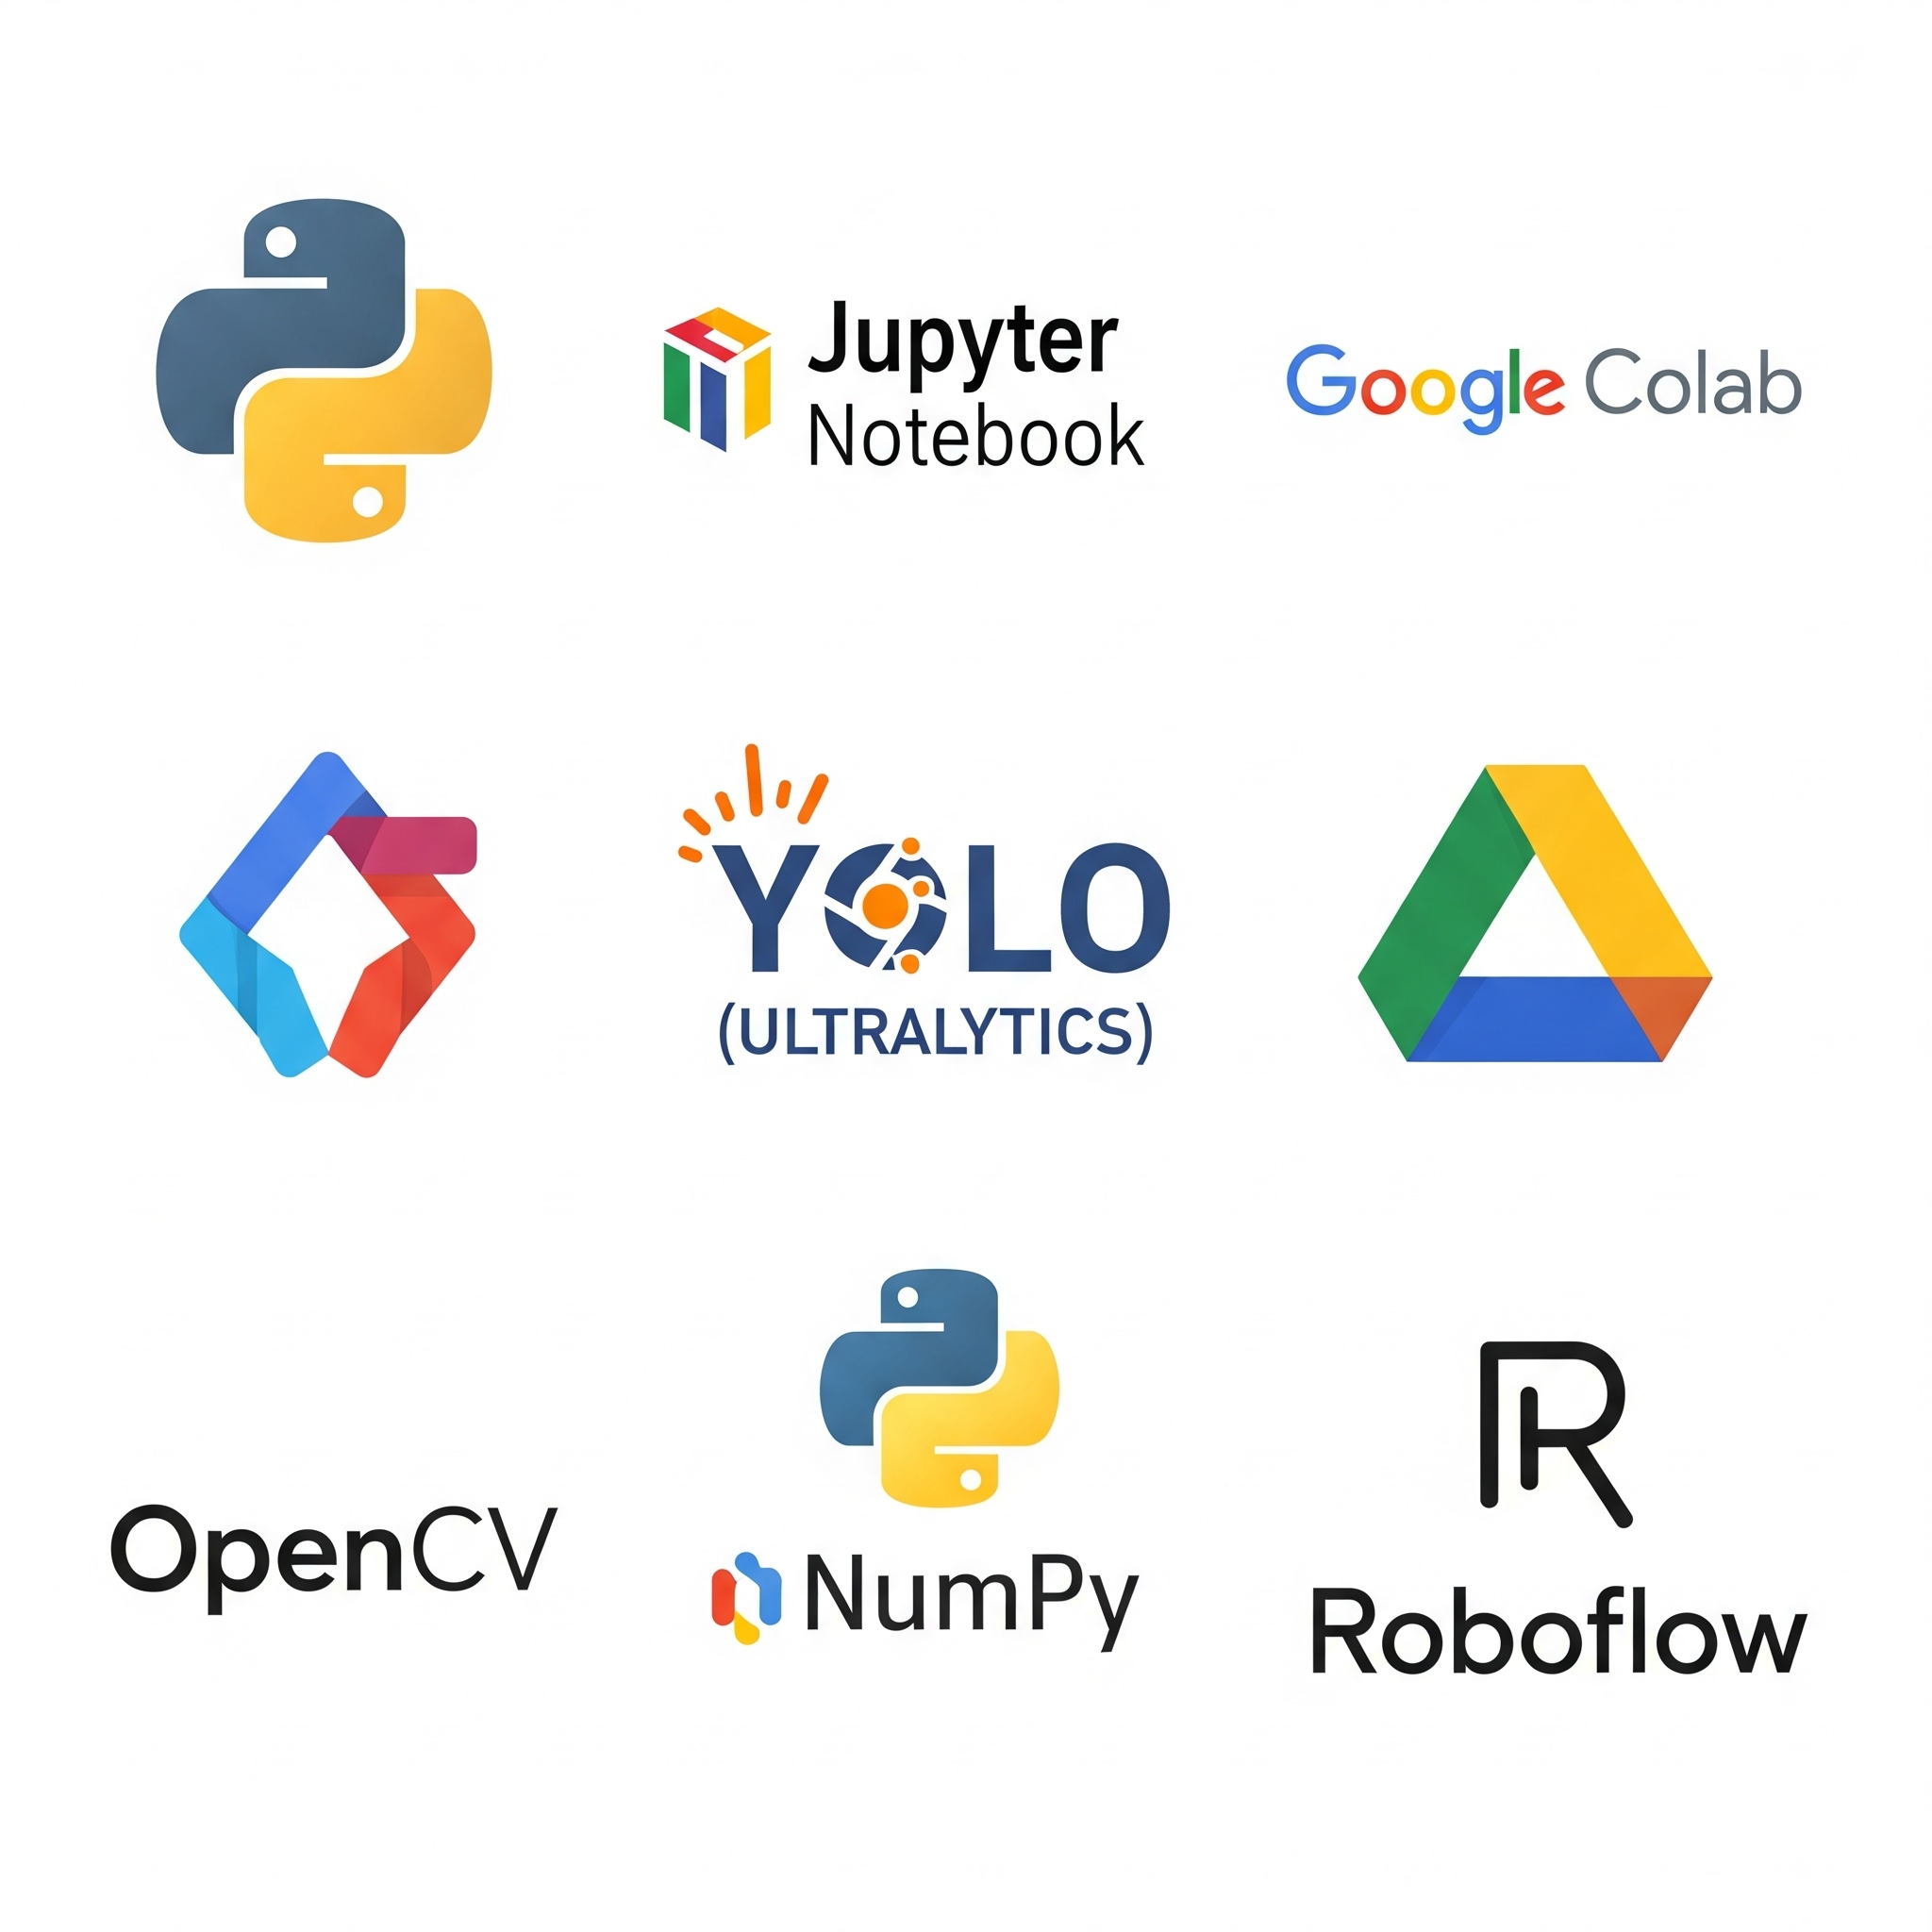
\includegraphics[width=0.6 \textwidth]{Figuras/tecnologias_logos.png}
  \\
  Fonte: Google Gemini.
  \label{fg-tecnologias-logos}
\end{figure}
% --- FIM Figura

\section{Coleta de Dados Visuais no Ambiente-Alvo}

A coleta de dados visuais é realizada no campus Pampulha da UFMG, ambiente escolhido por reunir circulação real de estudantes e variabilidade de cenários urbanos, como ruas internas, praças e paradas de ônibus. As gravações ocorrem em múltiplos dias e horários, abrangendo diferentes condições de luminosidade (manhã, tarde e noite) e de fluxo de pessoas, a fim de garantir diversidade nos dados. As Figuras \ref{fg-exe_grav_dia} e \ref{fg-exe_grav_noite} mostram exemplos diurnos e noturnos das fotos utilizadas.

% --- INÍCIO Figura
\begin{figure}[htbp]
  \centering
  \caption{Exemplo de foto diurna}
  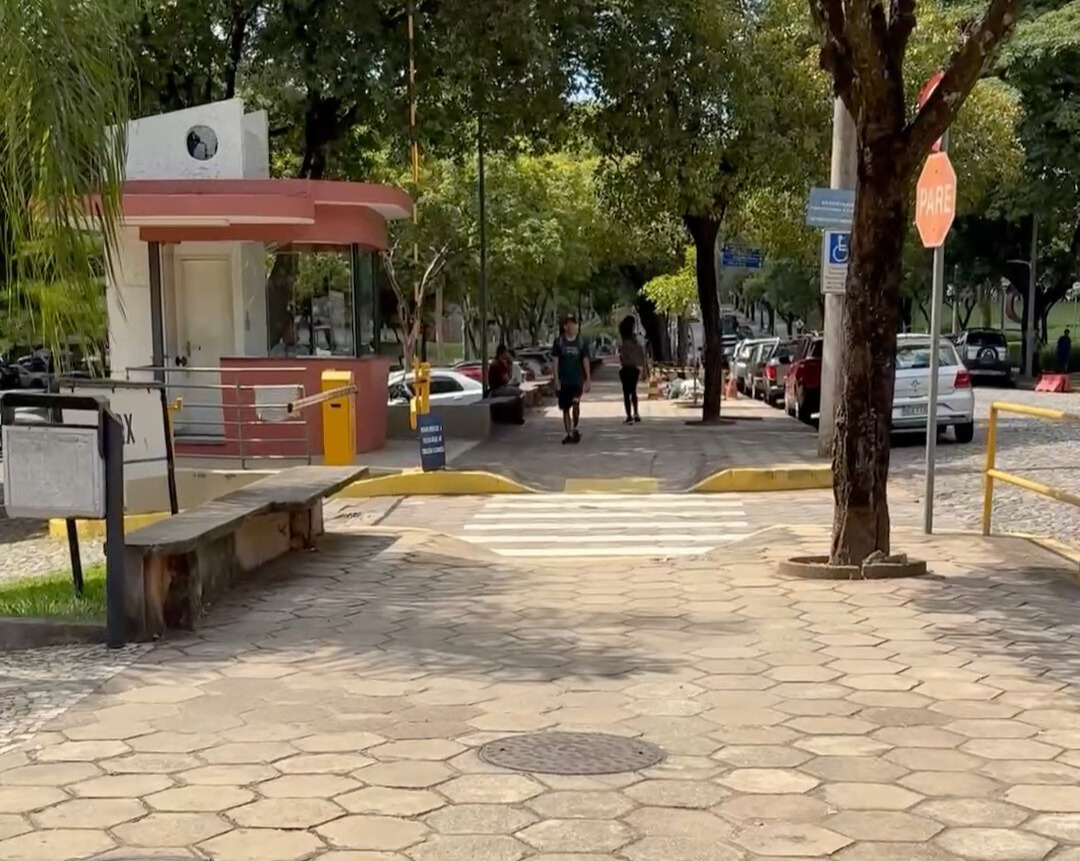
\includegraphics[width=0.8 \textwidth]{Figuras/exe_grav_dia - Editado.jpg}
  \\
  Fonte: Autoral.
  \label{fg-exe_grav_dia}
\end{figure}
% --- FIM Figura

% --- INÍCIO Figura
\begin{figure}[htbp]
  \centering
  \caption{Exemplo de foto noturna}
  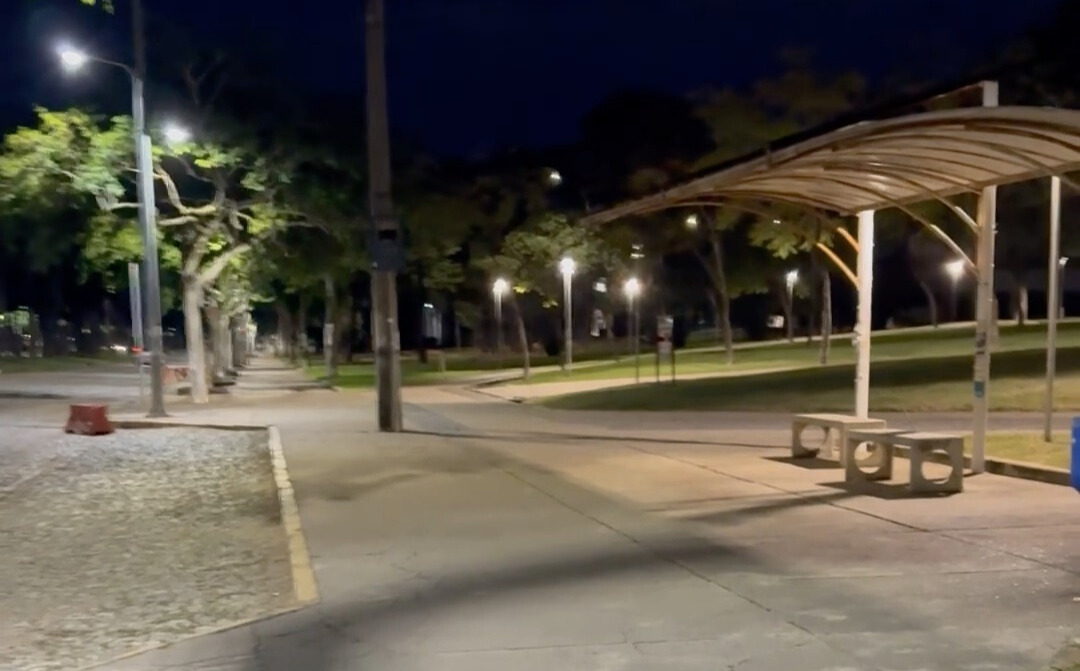
\includegraphics[width=0.8 \textwidth]{Figuras/exe_grav_noite - Editado.jpg}
  \\
  Fonte: Autoral.
  \label{fg-exe_grav_noite}
\end{figure}
% --- FIM Figura

Os vídeos são capturados com um smartphone posicionado na altura do peito, simulando a perspectiva de um usuário caminhando. Essa abordagem reproduz uma situação prática de uso em aplicações futuras. Todos os vídeos seguem configuração padronizada de resolução e taxa de quadros para manter consistência na captura.

Ao longo da coleta, são priorizados pontos do campus que contenham os três objetos de interesse: bancos, faixas de pedestre e placas de ponto de ônibus. A diversidade dos cenários permite treinar o modelo com diferentes formas, tamanhos e condições visuais dos objetos, incluindo situações com iluminação artificial, sombras acentuadas e obstruções parciais.

A extração de imagens dos vídeos é feita na plataforma Roboflow, resultando em aproximadamente 600 frames anotados. Cuidados éticos são tomados: evita-se focar em rostos ou informações pessoais, e os dados são usados exclusivamente para fins acadêmicos. Essa etapa assegura que o modelo seja treinado com dados realistas, aumentando sua robustez e aplicabilidade prática no mesmo ambiente onde será utilizado.

\section{Preparação do \textit{Dataset} Personalizado}

O dataset personalizado é construído com base em imagens extraídas dos vídeos gravados no campus Pampulha da UFMG. As três classes definidas para reconhecimento são: banco, faixa\_pedestre e placa\_onibus, escolhidas por sua relevância na navegação de pessoas com deficiência visual. Os frames são selecionados de forma a abranger diferentes horários do dia e níveis de ocupação do campus, garantindo diversidade nas condições de captura.

A anotação dos objetos é realizada manualmente na plataforma Roboflow, utilizando \textit{bounding boxes} para delimitar com precisão cada instância das classes de interesse. São anotadas mais de 600 imagens originais, com atenção à padronização dos nomes e ao formato das caixas, evitando inconsistências que possam prejudicar o aprendizado do modelo. As Figuras \ref{fg-ex_anot1}, \ref{fg-ex_anot2} e \ref{fg-ex_anot3} mostram exemplos de imagens anotadas no \textit{dataset} personalizado.

% --- INÍCIO Figura
\begin{figure}[htbp]
  \centering
  \caption{Exemplos de imagens com anotações realizadas}
  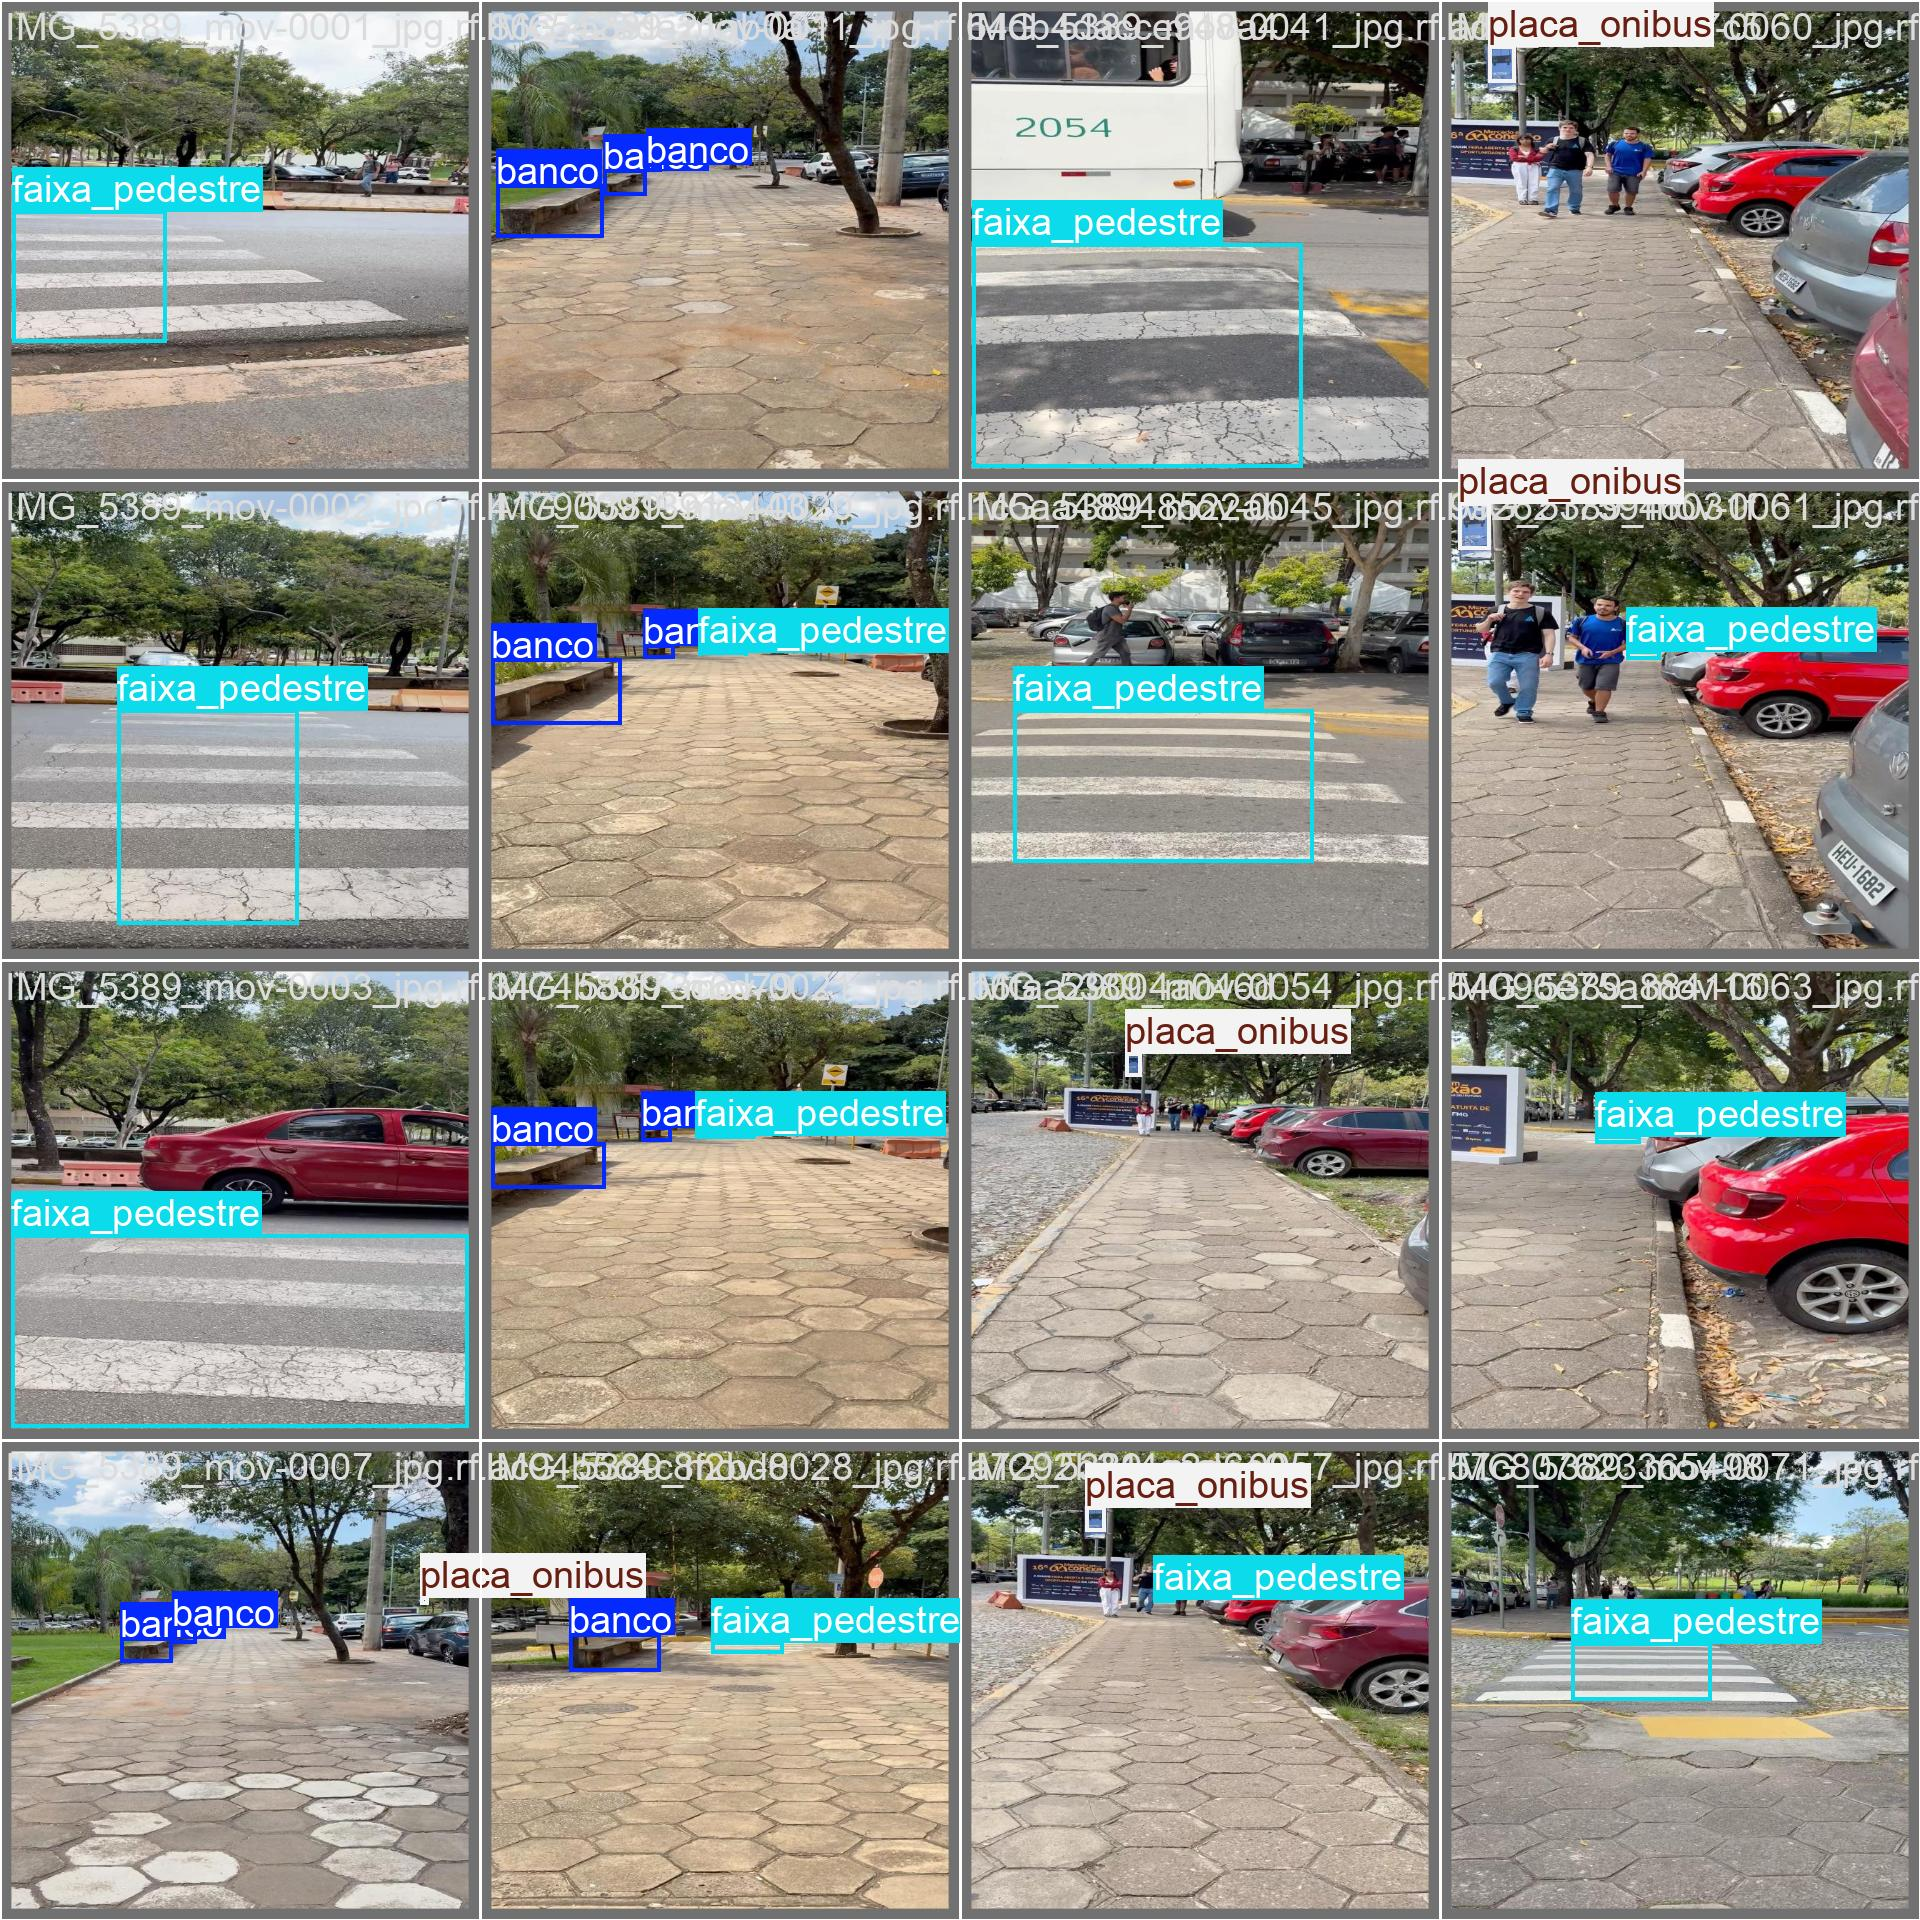
\includegraphics[width=1 \textwidth]{Figuras/val_batch0_labels.jpg}
  \\
  Fonte: Autoral.
  \label{fg-ex_anot1}
\end{figure}
% --- FIM Figura

% --- INÍCIO Figura
\begin{figure}[htbp]
  \centering
  \caption{Exemplos de imagens com anotações realizadas}
  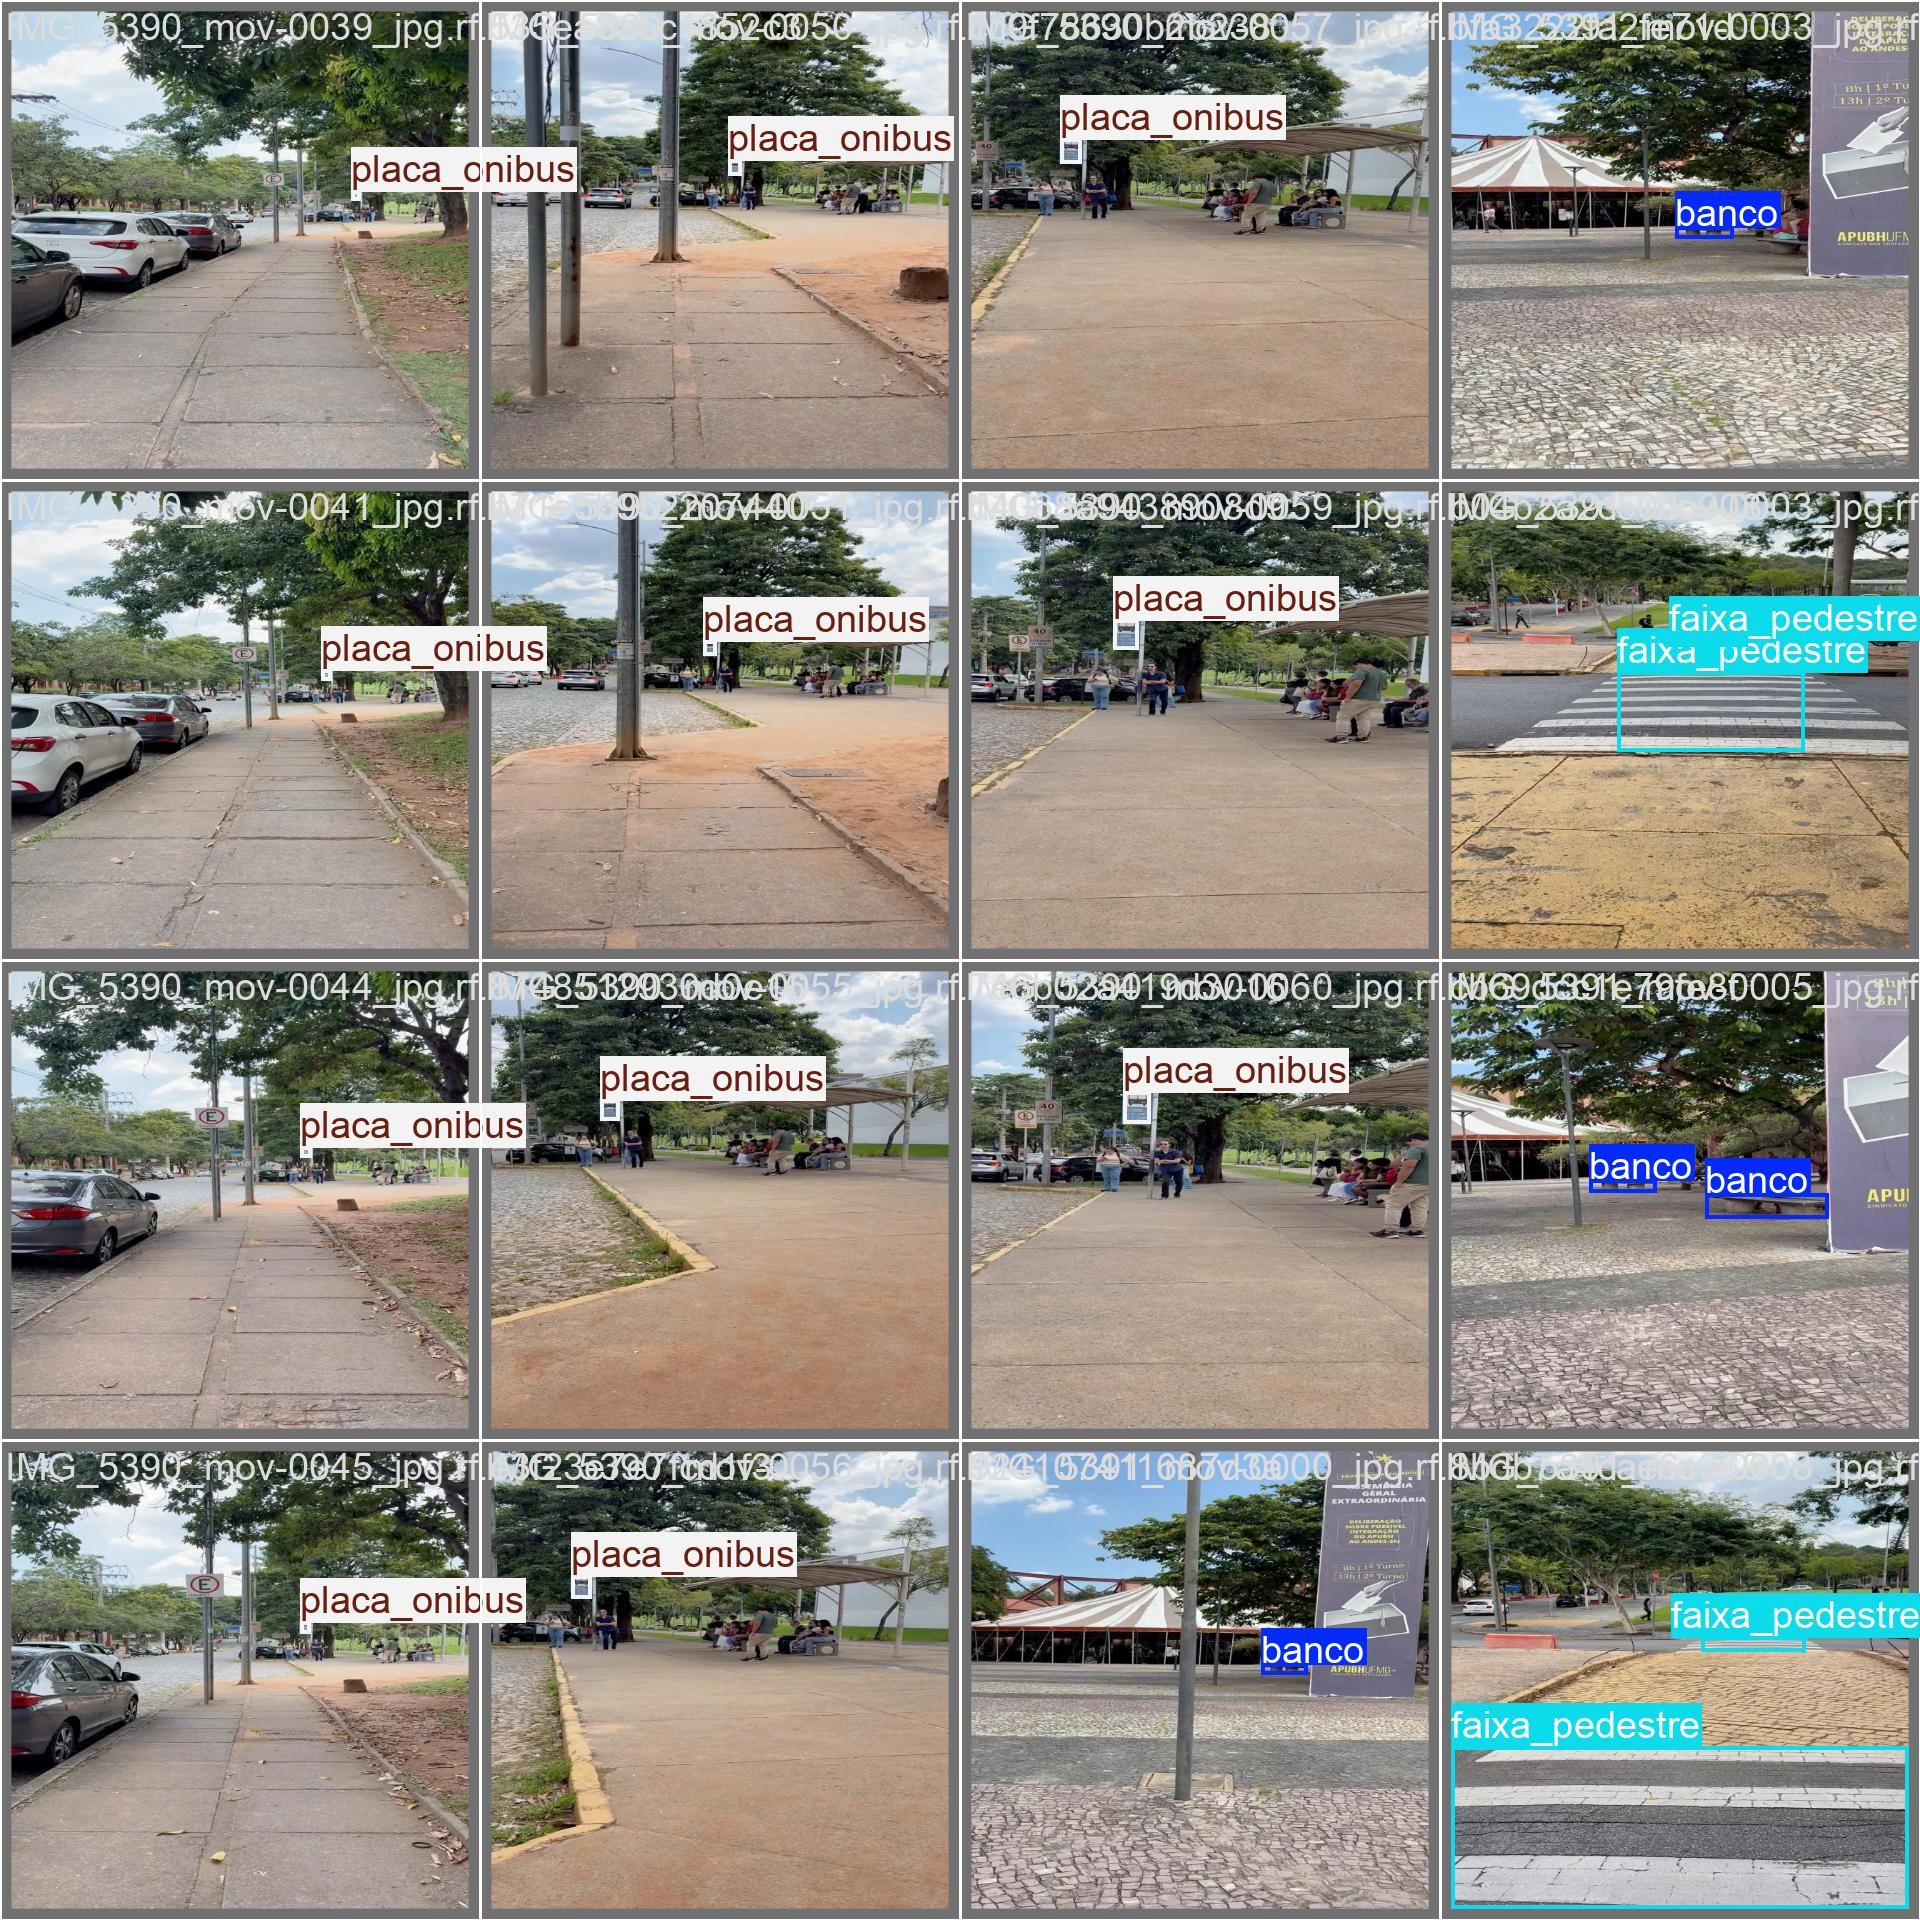
\includegraphics[width=1 \textwidth]{Figuras/val_batch1_labels.jpg}
  \\
  Fonte: Autoral.
  \label{fg-ex_anot2}
\end{figure}
% --- FIM Figura

% --- INÍCIO Figura
\begin{figure}[htbp]
  \centering
  \caption{Exemplos de imagens com anotações realizadas}
  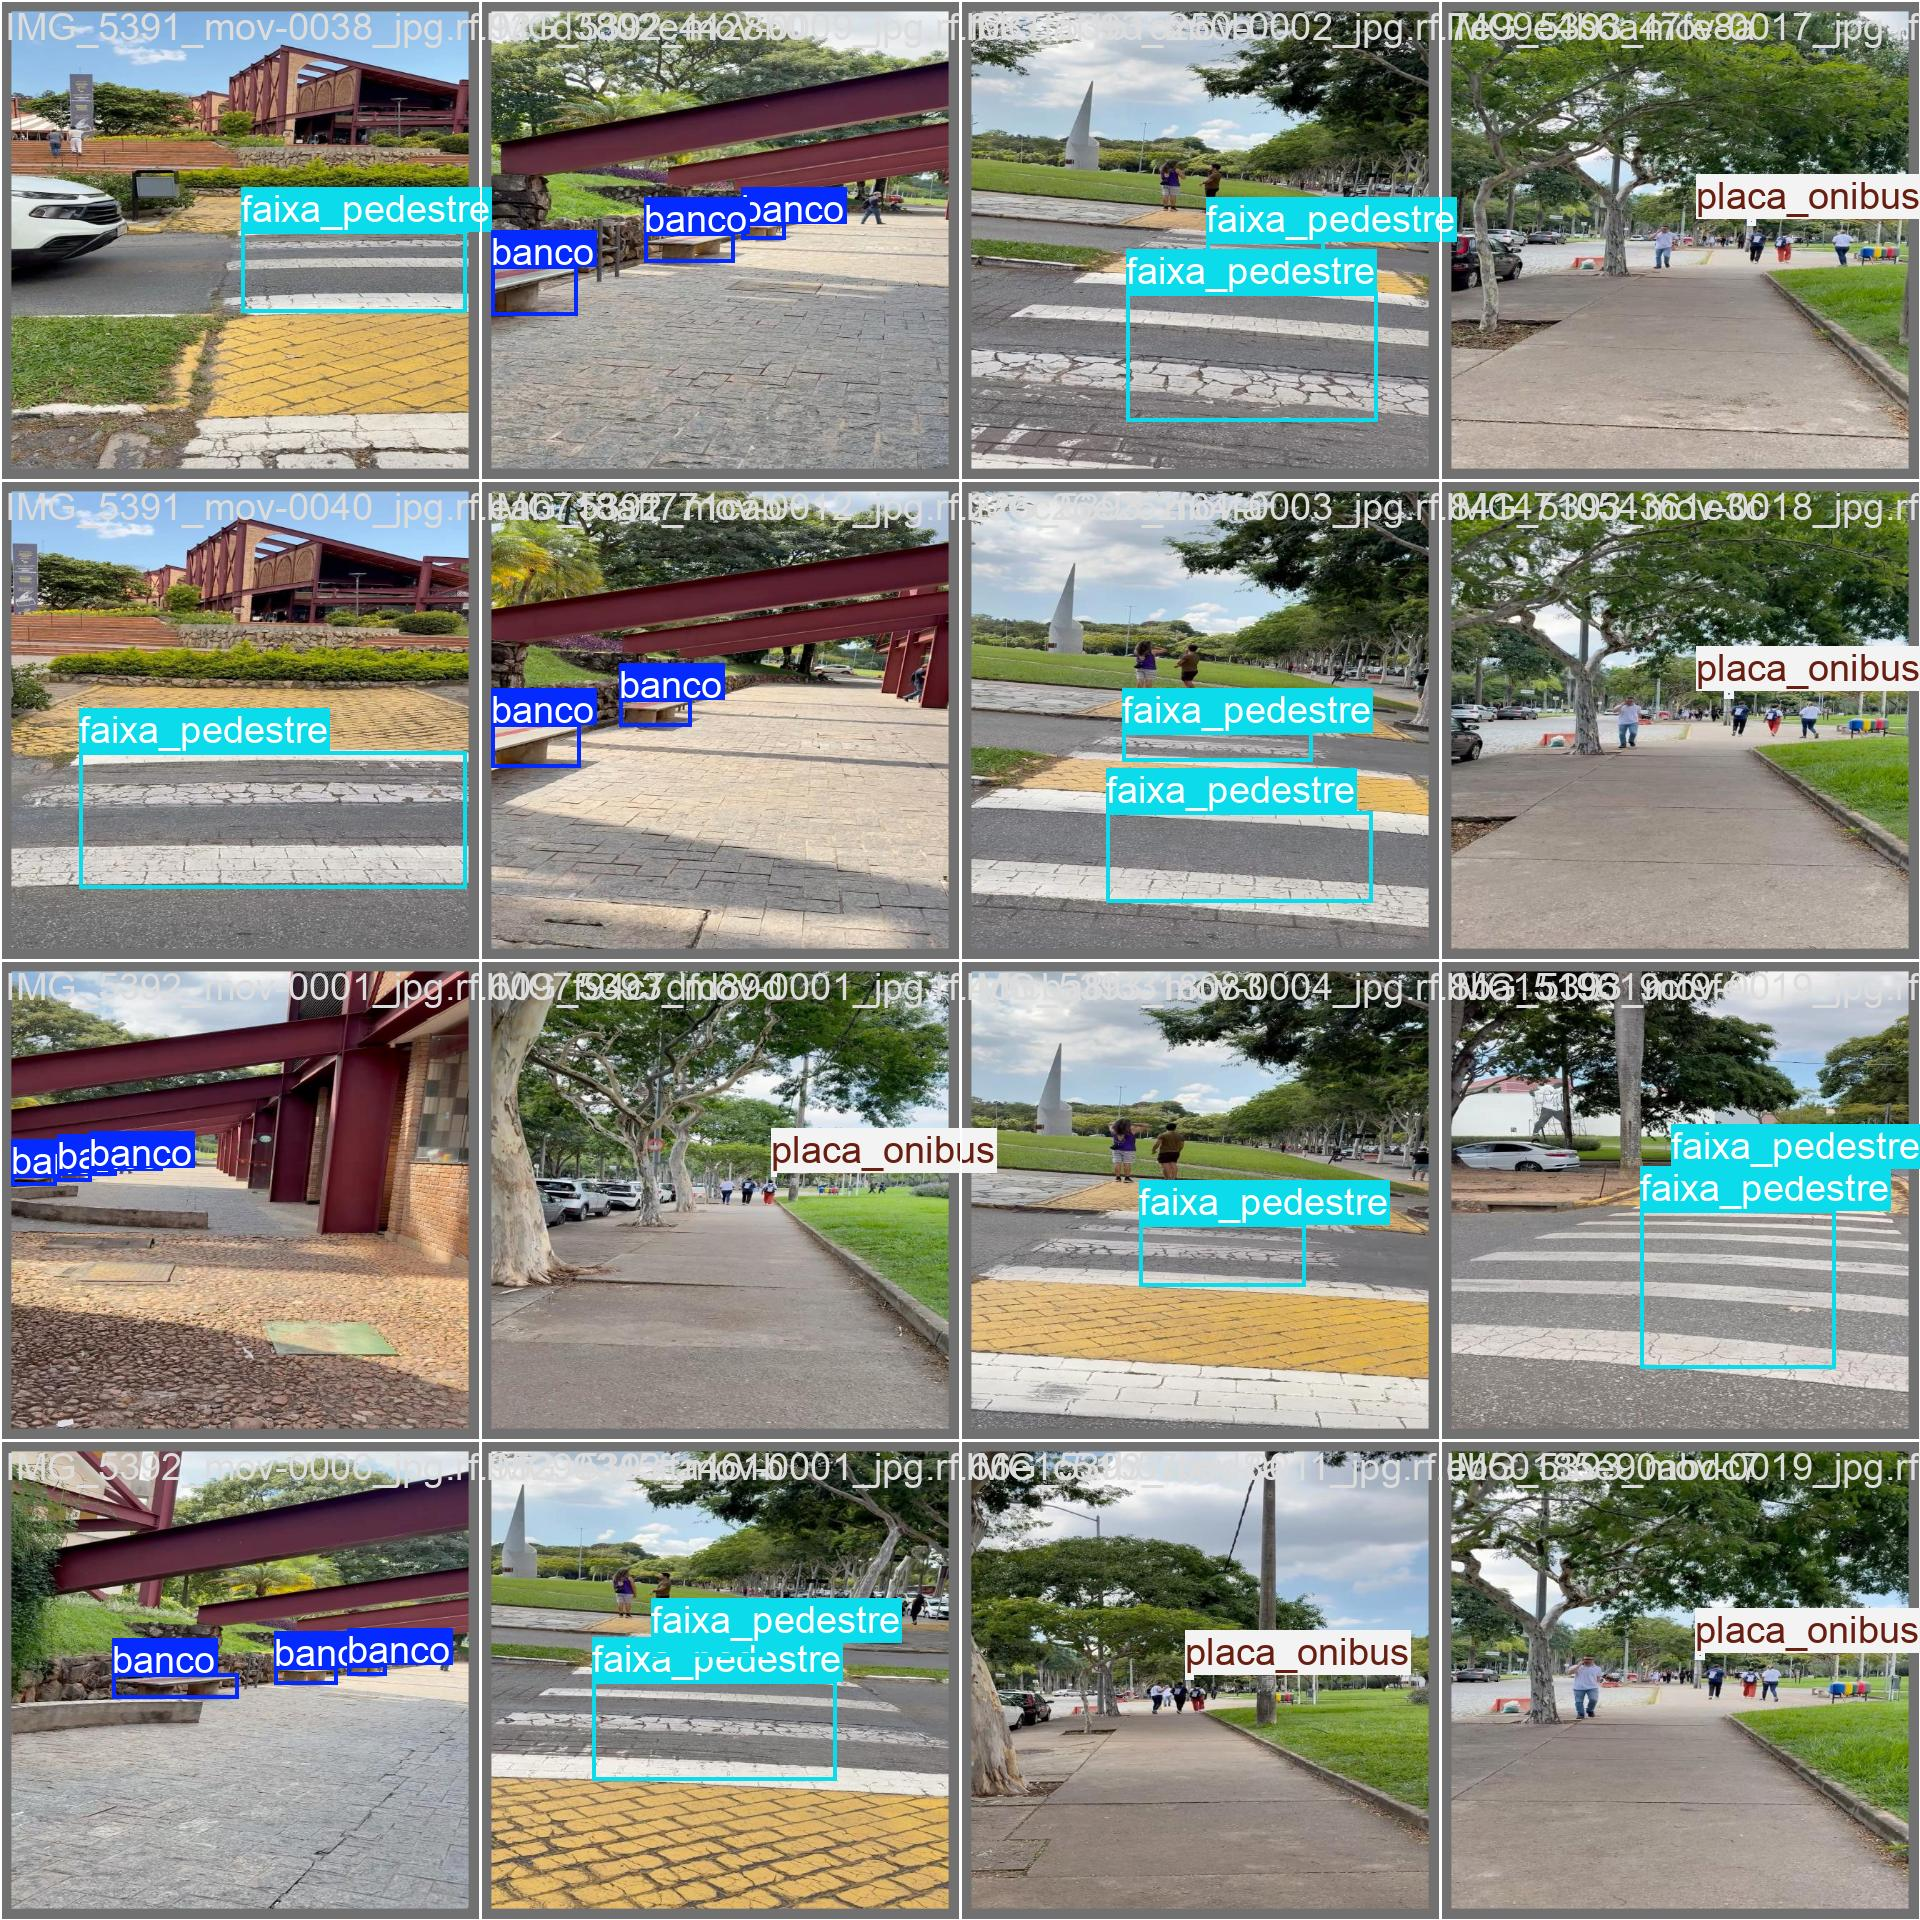
\includegraphics[width=1 \textwidth]{Figuras/val_batch2_labels.jpg}
  \\
  Fonte: Autoral.
  \label{fg-ex_anot3}
\end{figure}
% --- FIM Figura

Após a anotação, o dataset é expandido por meio de técnicas de \textit{data augmentation}, aplicando transformações como espelhamento, ajuste de brilho, saturação, ruído e \textit{blur}. Cada imagem gera três variações adicionais, elevando o número total para 1.444 imagens. Em seguida, os dados são redimensionados para 640x640 pixels e exportados no formato YOLO, com todos os arquivos organizados e enviados diretamente ao Google Colab via API.

A divisão final considera 88\% das imagens para treinamento e 12\% para validação, permitindo avaliar o desempenho durante o ajuste do modelo. A combinação de anotações precisas, variedade visual e aumentos realistas contribui para a robustez do modelo final, tornando essa etapa um dos pilares da qualidade do sistema proposto.

\section{Pré-processamento e \textit{Data Augmentation}}

As etapas de pré-processamento e \textit{data augmentation} são executadas diretamente na plataforma Roboflow, com o objetivo de padronizar e diversificar as imagens do dataset. Todas as imagens são redimensionadas para 640×640 pixels, formato exigido pelo modelo YOLOv11, e passam por um processo automático de auto-orientação, que corrige a rotação de imagens capturadas em ângulos variados.

O processo de \textit{data augmentation} introduz variações sintéticas que simulam diferentes condições reais de iluminação, perspectiva e qualidade de captura. São aplicadas as seguintes transformações: \textit{flip} horizontal, \textit{zoom} com \textit{crop} (até 15\%), \textit{shear} horizontal e vertical (±10°), variações de brilho, exposição, matiz e saturação, além de \textit{blur} (até 0.5px) e ruído (até 0.19\%). Essas alterações visam aumentar a robustez do modelo frente a cenários não vistos durante o treinamento.

Cada imagem anotada gera três novas variações, aumentando o número de exemplos de forma significativa. A plataforma Roboflow garante que todas as \textit{bounding boxes} sejam ajustadas corretamente após cada transformação, mantendo a integridade dos dados anotados. O resultado é um dataset balanceado, diversificado e com anotações consistentes, pronto para ser exportado no formato YOLO, com arquivos .txt e data.yaml.

Esse aumento sintético permite ampliar a capacidade de generalização do modelo mesmo com uma base original limitada. A aplicação de \textit{augmentations} realistas contribui diretamente para o bom desempenho do sistema em ambientes com diferentes condições de iluminação, movimento e visibilidade, como será evidenciado nos resultados.

\section{Treinamento do Modelo com o YOLOv11 personalizado}

O modelo é treinado a partir da arquitetura YOLOv11, utilizando como base o yolo11m.pt, fornecido pela Ultralytics. Essa versão apresenta um bom equilíbrio entre precisão e velocidade de inferência, sendo adequada para dispositivos com recursos computacionais moderados. O treinamento é realizado na plataforma Google Colab com GPU NVIDIA Tesla T4, utilizando Python 3.11.12 e a biblioteca oficial Ultralytics.

O dataset é importado diretamente da Roboflow via API, contendo imagens, anotações e o arquivo data.yaml. O treinamento é iniciado com o seguinte comando padrão:

!yolo task=detect mode=train data=data.yaml model="yolo11m.pt" epochs=80\\imgsz=640 batch=-1

Esse comando define a tarefa de detecção, usa o modelo base YOLOv11m, executa 80 épocas de treinamento com imagens de 640×640 pixels e deixa o batch size em modo automático. O modelo ajusta seus pesos com base em \textit{backpropagation} e otimização por gradiente, monitorando continuamente as perdas de caixas delimitadoras (box\_loss), classes (cls\_loss) e distribuição de distância de focal (dfl\_loss).

A cada época, o desempenho é validado com base nas métricas \textit{Precision}, \textit{Recall}, mAP@0.5 e mAP@0.5:0.95. O melhor modelo é salvo automaticamente em runs/detect/ufmg\_yolov11m\_run1/weights/best.pt. O processo completo leva menos de 1 hora, com estabilidade nas curvas de perda e sem indícios de \textit{overfitting}, o que indica que o modelo está generalizando bem para os dados de validação.

\section{Validação e Avaliação de Desempenho do Modelo}

A validação é conduzida com 12\% do conjunto de dados reservados exclusivamente para esse fim. Esse subconjunto inclui imagens em diferentes horários do dia, com variações de iluminação, distância e presença de oclusões parciais. O objetivo é verificar a capacidade de generalização do modelo YOLOv11 treinado e mensurar seu desempenho em condições realistas de uso.

A execução da validação é feita com o seguinte comando padrão:

!yolo task=detect mode=val model=best.pt data=data.yaml split=val

Os resultados incluem métricas padrão: \textit{Precision} (0.921), \textit{Recall} (0.915), mAP@0.5 (0.944) e mAP@0.5:0.95 (0.672). A performance por classe também é satisfatória, com destaque para “placa\_onibus”, que atinge \textit{Precision} de 1.000 e \textit{Recall} de 0.997. A classe “banco” apresenta desempenho ligeiramente inferior (mAP@0.5:0.95 de 0.615), influenciada por oclusões e variações visuais nos vídeos.

O tempo médio de inferência é de 29,1 ms por imagem, com pré-processamento em torno de 4,0 ms e pós-processamento de 4,8 ms, demonstrando viabilidade para aplicações em tempo quase real. As curvas de perda e gráficos de desempenho gerados pela biblioteca Ultralytics mostram uma convergência estável sem indícios de overfitting. Também é realizada uma validação qualitativa com novos vídeos capturados no campus, confirmando a precisão das detecções em ambientes não vistos pelo modelo.

\section{Testes em Vídeos Reais e Análise Qualitativa}

Para avaliar o desempenho do sistema em condições reais de uso, são realizados testes com vídeos distintos dos utilizados no treinamento e validação. As gravações são feitas com o celular preso à altura do peito, simulando a perspectiva de um usuário durante o deslocamento no campus Pampulha da UFMG. Os testes abrangem diferentes horários do dia, condições de iluminação e variação de ocupação do ambiente.

A análise qualitativa baseia-se na observação visual das detecções renderizadas sobre os vídeos. São avaliados a estabilidade das \textit{bounding boxes}, a consistência na classificação dos objetos e a robustez diante de oclusões, movimentações no cenário e variações de luz. O modelo mantém boa performance geral, com confiabilidade superior a 0.85 em grande parte dos quadros para as classes placa\_onibus e faixa\_pedestre. A classe banco apresenta maior sensibilidade a obstáculos visuais, como presença de pessoas ou vegetação.

Além das detecções visuais, também é testado o funcionamento do sistema de geração de alertas sonoros. Os áudios, sincronizados aos vídeos, transmitem informações contextuais com clareza e precisão. A integração entre detecção visual e feedback auditivo reforça o potencial da ferramenta para aplicações assistivas, demonstrando fluidez na comunicação com o usuário.

As limitações observadas incluem quedas na confiança durante cenas noturnas ou com iluminação artificial intensa, além de falhas pontuais na detecção de objetos em ângulos extremos. Apesar disso, os testes confirmam que o sistema é funcional em contextos diversos, com desempenho robusto e usabilidade promissora, servindo como prova de conceito viável para aplicações futuras em tempo real.

\section{Geração de \textit{Feedback} Auditivo a partir das Detecções}

Nesta etapa, o sistema converte as detecções visuais em mensagens sonoras, possibilitando que pessoas com deficiência visual compreendam a presença e a localização de objetos no ambiente. A conversão é feita com a biblioteca gTTS, que transforma textos em áudios no idioma português. A cada detecção válida, o sistema gera frases como “faixa de pedestre à frente” ou “banco à esquerda”, que são sincronizadas com o vídeo correspondente.

Para determinar a posição dos objetos, o sistema divide cada \textit{frame} em três regiões verticais (esquerda, centro e direita), com base no ponto central da \textit{bounding box} detectada. Um deslocamento percentual de 15\% dos \textit{pixels} a partir do centro define os limites laterais. A partir da classe e da posição, o sistema concatena a string da mensagem que será convertida em áudio.

O áudio gerado é sincronizado com os frames do vídeo utilizando a biblioteca MoviePy, enquanto o módulo de \textit{debouncing} evita repetição de alertas em posições semelhantes em curto intervalo de tempo. Os limiares de repetição são ajustados conforme a classe: placas de ponto de ônibus e faixas exigem maior espaçamento, enquanto bancos admitem menor intervalo.

O processamento final gera um vídeo com detecções visuais sobrepostas e alertas sonoros integrados, simulando o uso real do sistema. Toda a implementação é feita em Python, com as bibliotecas Ultralytics, OpenCV, gTTS, MoviePy, NumPy e logging. O código está disponível no GitHub\footnote{\url{https://github.com/seu-usuario/seu-repositorio}} e modularizado para facilitar manutenção e reuso. O resultado demonstra que o sistema é capaz de traduzir informações visuais em mensagens acessíveis, aproximando-se de uma solução funcional de tecnologia assistiva.

\section{Considerações Éticas e Limitações da Implementação}

A coleta de dados visuais é realizada exclusivamente em áreas públicas do campus Pampulha da UFMG, com foco em objetos de interesse definidos previamente. O projeto evita a identificação de pessoas e não armazena dados sensíveis. Em casos em que indivíduos aparecem incidentalmente nos vídeos, não ocorre qualquer tentativa de reconhecimento facial ou extração de informações pessoais, e as imagens são utilizadas apenas para treinamento interno do modelo.

A proposta busca ampliar a acessibilidade para pessoas com deficiência visual, respeitando diretrizes éticas e legais. A solução é concebida como uma ferramenta de baixo custo, com potencial para ser embarcada em dispositivos móveis e adaptada a outros contextos institucionais ou urbanos. A finalidade do sistema é exclusivamente assistiva, sem coleta de dados do usuário ou uso comercial das imagens.

Entre as principais limitações, destaca-se o fato de que o sistema opera com vídeos pré-gravados, e não em tempo real. Isso impede seu uso imediato como ferramenta interativa e exige processamento posterior para gerar os alertas. A implementação em tempo real requer dispositivos com maior capacidade computacional e ajustes na integração com câmeras em execução contínua. Além disso, o modelo é treinado com dados específicos do campus da UFMG, o que pode reduzir sua precisão em outros contextos, como ruas urbanas ou outras instituições.

Variações ambientais, como baixa iluminação, obstruções visuais e mudanças climáticas, também impactam a confiabilidade do sistema. O posicionamento da câmera no corpo do usuário pode gerar distorções na detecção, exigindo padronização ou mecanismos adaptativos. Embora os testes realizados indiquem bons resultados, a validação com usuários reais ainda é necessária para aferir a clareza dos alertas, o conforto auditivo e a efetividade da solução em situações cotidianas.

\section{Estrutura de Arquivos, \textit{Logs} e Reprodutibilidade}

O projeto é organizado em uma estrutura de pastas que favorece a reprodutibilidade, o versionamento dos resultados e a clareza nas etapas de execução. Quatro diretórios principais são utilizados: /scripts, que contém todos os códigos-fonte em Python divididos por função (treinamento, validação, inferência, feedback auditivo e montagem final de vídeos); /datasets, que armazena as imagens e anotações em formato YOLO organizadas nas pastas train/ e val/; /runs, onde a biblioteca Ultralytics salva automaticamente os pesos dos modelos e os logs de desempenho; e /outputs, que concentra os vídeos processados, com e sem áudio.

Além desses, é criada a pasta /logs, destinada ao armazenamento dos arquivos .log gerados pela biblioteca logging. Cada execução registra \textit{timestamp}, classe detectada, nível de confiança e posição relativa dos objetos (esquerda, centro ou direita). Esses registros possibilitam auditoria dos resultados, análise estatística posterior e identificação de falhas de detecção ou inconsistência no feedback auditivo.

O código é modularizado em \textit{scripts} independentes com parâmetros personalizáveis, favorecendo o reaproveitamento por outros usuários. Cada função do sistema, desde a importação do \textit{dataset} até a geração do vídeo final com feedback auditivo, está encapsulada em células distintas no Jupyter Notebook, com comentários explicativos e exemplos de uso. Essa abordagem facilita a reprodução dos experimentos por terceiros com mínimas alterações, como a troca de vídeos ou modelos de detecção.

O repositório público do projeto no GitHub inclui um arquivo README.md com instruções detalhadas de instalação e uso, além de um requirements.txt que lista todas as bibliotecas utilizadas (incluindo ultralytics, opencv-python, gtts, moviepy, numpy e torch, entre outras). Todos os testes são conduzidos no Google Colab com configuração consistente de ambiente, garantindo que o experimento possa ser replicado fielmente. Essa estrutura de organização e documentação é um diferencial que assegura a validade metodológica do trabalho e contribui para sua disseminação acadêmica.

\section{Considerações Finais}

Este trabalho adota uma abordagem aplicada e experimental, com foco na construção de uma solução funcional voltada à assistência de pessoas com deficiência visual no campus da UFMG. A proposta parte de um problema real e busca resolvê-lo com o uso de tecnologias existentes, integradas de forma prática, iterativa e mensurável.

A metodologia desenvolvida segue uma lógica incremental, em que cada etapa, desde a coleta dos dados até a geração de feedback auditivo, contribui de forma objetiva para a composição de um sistema funcional. O modelo treinado é testado com vídeos reais, anotados manualmente, e os resultados são validados por métricas quantitativas e por testes qualitativos em condições variadas de uso. Essa abordagem permite verificar não apenas a precisão algorítmica, mas também a adequação funcional do sistema no ambiente-alvo.

Do ponto de vista técnico, o trabalho se destaca por utilizar ferramentas de código aberto e infraestrutura gratuita (Google Colab, Roboflow, Ultralytics), promovendo reprodutibilidade, acessibilidade e escalabilidade. As decisões metodológicas priorizam a clareza, a leveza computacional e a adaptabilidade a diferentes contextos futuros, mesmo com recursos limitados.

Por fim, o trabalho propõe mais do que um experimento acadêmico: apresenta uma prova de conceito concreta, replicável e socialmente relevante. A estratégia adotada demonstra que é possível construir sistemas assistivos eficientes com tecnologias atuais e acessíveis, desde que com planejamento metodológico sólido e foco nas reais necessidades do público-alvo.